\documentclass[twoside]{book}

% Packages required by doxygen
\usepackage{calc}
\usepackage{doxygen}
\usepackage{graphicx}
\usepackage[utf8]{inputenc}
\usepackage{makeidx}
\usepackage{multicol}
\usepackage{multirow}
\usepackage{textcomp}
\usepackage[table]{xcolor}

% NLS support packages
\usepackage{hfont}

% Font selection
\usepackage[T1]{fontenc}
\usepackage{mathptmx}
\usepackage[scaled=.90]{helvet}
\usepackage{courier}
\usepackage{amssymb}
\usepackage{sectsty}
\renewcommand{\familydefault}{\sfdefault}
\allsectionsfont{%
  \fontseries{bc}\selectfont%
  \color{darkgray}%
}
\renewcommand{\DoxyLabelFont}{%
  \fontseries{bc}\selectfont%
  \color{darkgray}%
}

% Page & text layout
\usepackage{geometry}
\geometry{%
  a4paper,%
  top=2.5cm,%
  bottom=2.5cm,%
  left=2.5cm,%
  right=2.5cm%
}
\tolerance=750
\hfuzz=15pt
\hbadness=750
\setlength{\emergencystretch}{15pt}
\setlength{\parindent}{0cm}
\setlength{\parskip}{0.2cm}
\makeatletter
\renewcommand{\paragraph}{%
  \@startsection{paragraph}{4}{0ex}{-1.0ex}{1.0ex}{%
    \normalfont\normalsize\bfseries\SS@parafont%
  }%
}
\renewcommand{\subparagraph}{%
  \@startsection{subparagraph}{5}{0ex}{-1.0ex}{1.0ex}{%
    \normalfont\normalsize\bfseries\SS@subparafont%
  }%
}
\makeatother

% Headers & footers
\usepackage{fancyhdr}
\pagestyle{fancyplain}
\fancyhead[LE]{\fancyplain{}{\bfseries\thepage}}
\fancyhead[CE]{\fancyplain{}{}}
\fancyhead[RE]{\fancyplain{}{\bfseries\leftmark}}
\fancyhead[LO]{\fancyplain{}{\bfseries\rightmark}}
\fancyhead[CO]{\fancyplain{}{}}
\fancyhead[RO]{\fancyplain{}{\bfseries\thepage}}
\fancyfoot[LE]{\fancyplain{}{}}
\fancyfoot[CE]{\fancyplain{}{}}
\fancyfoot[RE]{\fancyplain{}{\bfseries\scriptsize 생성시간 \-: 화 12월 31 2013 07\-:11\-:12, 프로젝트명 \-: Reactor, 생성자 \-:  Doxygen }}
\fancyfoot[LO]{\fancyplain{}{\bfseries\scriptsize 생성시간 \-: 화 12월 31 2013 07\-:11\-:12, 프로젝트명 \-: Reactor, 생성자 \-:  Doxygen }}
\fancyfoot[CO]{\fancyplain{}{}}
\fancyfoot[RO]{\fancyplain{}{}}
\renewcommand{\footrulewidth}{0.4pt}
\renewcommand{\chaptermark}[1]{%
  \markboth{#1}{}%
}
\renewcommand{\sectionmark}[1]{%
  \markright{\thesection\ #1}%
}

% Indices & bibliography
\usepackage{natbib}
\usepackage[titles]{tocloft}
\setcounter{tocdepth}{3}
\setcounter{secnumdepth}{5}
\makeindex

% Hyperlinks (required, but should be loaded last)
\usepackage{ifpdf}
\ifpdf
  \usepackage[pdftex,pagebackref=true]{hyperref}
\else
  \usepackage[ps2pdf,pagebackref=true]{hyperref}
\fi
\hypersetup{%
  colorlinks=true,%
  linkcolor=blue,%
  citecolor=blue,%
  unicode%
}

% Custom commands
\newcommand{\clearemptydoublepage}{%
  \newpage{\pagestyle{empty}\cleardoublepage}%
}


%===== C O N T E N T S =====

\begin{document}

% Titlepage & ToC
\hypersetup{pageanchor=false}
\pagenumbering{roman}
\begin{titlepage}
\vspace*{7cm}
\begin{center}%
{\Large Reactor \\[1ex]\large 1.\-0.\-0 }\\
\vspace*{1cm}
{\large 다음에 의해 생성됨 \-:  Doxygen 1.8.6}\\
\vspace*{0.5cm}
{\small 화 12월 31 2013 07:11:12}\\
\end{center}
\end{titlepage}
\clearemptydoublepage
\tableofcontents
\clearemptydoublepage
\pagenumbering{arabic}
\hypersetup{pageanchor=true}

%--- Begin generated contents ---
\chapter{네임스페이스 색인}
\section{패키지}
다음은 패키지들입니다. (가능한한 간략한 설명만을 보여줍니다) \-:\begin{DoxyCompactList}
\item\contentsline{section}{\hyperlink{namespaceclient}{client} }{\pageref{namespaceclient}}{}
\item\contentsline{section}{\hyperlink{namespaceserver}{server} }{\pageref{namespaceserver}}{}
\item\contentsline{section}{\hyperlink{namespaceserver_1_1event__handler}{server.\-event\-\_\-handler} }{\pageref{namespaceserver_1_1event__handler}}{}
\end{DoxyCompactList}

\chapter{계통도 색인}
\section{클래스 계통도}
이 상속 목록은 완전하진 않지만 알파벳순으로 대략적으로 정렬되어있습니다.\-:\begin{DoxyCompactList}
\item \contentsline{section}{server.\-Demultiplexer}{\pageref{classserver_1_1_demultiplexer}}{}
\item \contentsline{section}{server.\-event\-\_\-handler.\-Event\-Handler}{\pageref{classserver_1_1event__handler_1_1_event_handler}}{}
\begin{DoxyCompactList}
\item \contentsline{section}{server.\-event\-\_\-handler.\-A\-Event\-Handler}{\pageref{classserver_1_1event__handler_1_1_a_event_handler}}{}
\item \contentsline{section}{server.\-event\-\_\-handler.\-B\-Event\-Handler}{\pageref{classserver_1_1event__handler_1_1_b_event_handler}}{}
\end{DoxyCompactList}
\item \contentsline{section}{client.\-Main}{\pageref{classclient_1_1_main}}{}
\item \contentsline{section}{server.\-Reactor}{\pageref{classserver_1_1_reactor}}{}
\item \contentsline{section}{server.\-Server\-Initialize}{\pageref{classserver_1_1_server_initialize}}{}
\item Hash\-Map\begin{DoxyCompactList}
\item \contentsline{section}{server.\-Handle\-Map}{\pageref{classserver_1_1_handle_map}}{}
\end{DoxyCompactList}
\end{DoxyCompactList}

\chapter{클래스 색인}
\section{클래스 목록}
다음은 클래스, 구조체, 공용체 그리고 인터페이스들입니다. (간략한 설명만을 보여줍니다) \-:\begin{DoxyCompactList}
\item\contentsline{section}{\hyperlink{classserver_1_1event__handler_1_1_a_event_handler}{server.\-event\-\_\-handler.\-A\-Event\-Handler} }{\pageref{classserver_1_1event__handler_1_1_a_event_handler}}{}
\item\contentsline{section}{\hyperlink{classserver_1_1event__handler_1_1_b_event_handler}{server.\-event\-\_\-handler.\-B\-Event\-Handler} }{\pageref{classserver_1_1event__handler_1_1_b_event_handler}}{}
\item\contentsline{section}{\hyperlink{classserver_1_1_demultiplexer}{server.\-Demultiplexer} }{\pageref{classserver_1_1_demultiplexer}}{}
\item\contentsline{section}{\hyperlink{classserver_1_1event__handler_1_1_event_handler}{server.\-event\-\_\-handler.\-Event\-Handler} }{\pageref{classserver_1_1event__handler_1_1_event_handler}}{}
\item\contentsline{section}{\hyperlink{classserver_1_1_handle_map}{server.\-Handle\-Map} }{\pageref{classserver_1_1_handle_map}}{}
\item\contentsline{section}{\hyperlink{classclient_1_1_main}{client.\-Main} }{\pageref{classclient_1_1_main}}{}
\item\contentsline{section}{\hyperlink{classserver_1_1_reactor}{server.\-Reactor} }{\pageref{classserver_1_1_reactor}}{}
\item\contentsline{section}{\hyperlink{classserver_1_1_server_initialize}{server.\-Server\-Initialize} }{\pageref{classserver_1_1_server_initialize}}{}
\end{DoxyCompactList}

\chapter{파일 색인}
\section{파일 목록}
다음은 모든 파일에 대한 목록입니다. (간략한 설명만을 보여줍니다) \-:\begin{DoxyCompactList}
\item\contentsline{section}{src/client/\hyperlink{_main_8java}{Main.\-java} }{\pageref{_main_8java}}{}
\item\contentsline{section}{src/server/\hyperlink{_demultiplexer_8java}{Demultiplexer.\-java} }{\pageref{_demultiplexer_8java}}{}
\item\contentsline{section}{src/server/\hyperlink{_handle_map_8java}{Handle\-Map.\-java} }{\pageref{_handle_map_8java}}{}
\item\contentsline{section}{src/server/\hyperlink{_reactor_8java}{Reactor.\-java} }{\pageref{_reactor_8java}}{}
\item\contentsline{section}{src/server/\hyperlink{_server_initialize_8java}{Server\-Initialize.\-java} }{\pageref{_server_initialize_8java}}{}
\item\contentsline{section}{src/server/event\-\_\-handler/\hyperlink{_a_event_handler_8java}{A\-Event\-Handler.\-java} }{\pageref{_a_event_handler_8java}}{}
\item\contentsline{section}{src/server/event\-\_\-handler/\hyperlink{_b_event_handler_8java}{B\-Event\-Handler.\-java} }{\pageref{_b_event_handler_8java}}{}
\item\contentsline{section}{src/server/event\-\_\-handler/\hyperlink{_event_handler_8java}{Event\-Handler.\-java} }{\pageref{_event_handler_8java}}{}
\end{DoxyCompactList}

\chapter{네임스페이스 문서화}
\hypertarget{namespaceclient}{\section{client 패키지}
\label{namespaceclient}\index{client@{client}}
}
\subsection*{클래스}
\begin{DoxyCompactItemize}
\item 
class \hyperlink{classclient_1_1_main}{Main}
\end{DoxyCompactItemize}

\hypertarget{namespaceserver}{\section{server 패키지}
\label{namespaceserver}\index{server@{server}}
}
\subsection*{패키지}
\begin{DoxyCompactItemize}
\item 
package \hyperlink{namespaceserver_1_1event__handler}{event\-\_\-handler}
\begin{DoxyCompactList}\small\item\em alkjsdf \end{DoxyCompactList}\end{DoxyCompactItemize}
\subsection*{클래스}
\begin{DoxyCompactItemize}
\item 
class \hyperlink{classserver_1_1_demultiplexer}{Demultiplexer}
\begin{DoxyCompactList}\small\item\em 이벤트를 디코딩하여 적절한 핸들러에 전달한다. \end{DoxyCompactList}\item 
class \hyperlink{classserver_1_1_handle_map}{Handle\-Map}
\begin{DoxyCompactList}\small\item\em 핸들과 이벤트 핸들러를 해쉬 형태로 저장하는 객체. \end{DoxyCompactList}\item 
class \hyperlink{classserver_1_1_reactor}{Reactor}
\begin{DoxyCompactList}\small\item\em 이벤트 핸들러를 관리하는 객체. \end{DoxyCompactList}\item 
class \hyperlink{classserver_1_1_server_initialize}{Server\-Initialize}
\begin{DoxyCompactList}\small\item\em 서버 초기화 클래스 \end{DoxyCompactList}\end{DoxyCompactItemize}

\hypertarget{namespaceserver_1_1event__handler}{\section{server.\-event\-\_\-handler 패키지}
\label{namespaceserver_1_1event__handler}\index{server.\-event\-\_\-handler@{server.\-event\-\_\-handler}}
}
\subsection*{클래스}
\begin{DoxyCompactItemize}
\item 
class \hyperlink{classserver_1_1event__handler_1_1_a_event_handler}{A\-Event\-Handler}
\item 
class \hyperlink{classserver_1_1event__handler_1_1_b_event_handler}{B\-Event\-Handler}
\item 
class \hyperlink{classserver_1_1event__handler_1_1_event_handler}{Event\-Handler}
\end{DoxyCompactItemize}

\chapter{클래스 문서화}
\hypertarget{classserver_1_1event__handler_1_1_a_event_handler}{\section{server.\-event\-\_\-handler.\-A\-Event\-Handler 클래스 참조}
\label{classserver_1_1event__handler_1_1_a_event_handler}\index{server.\-event\-\_\-handler.\-A\-Event\-Handler@{server.\-event\-\_\-handler.\-A\-Event\-Handler}}
}


server.\-event\-\_\-handler.\-A\-Event\-Handler에 대한 상속 다이어그램 \-: 
\nopagebreak
\begin{figure}[H]
\begin{center}
\leavevmode
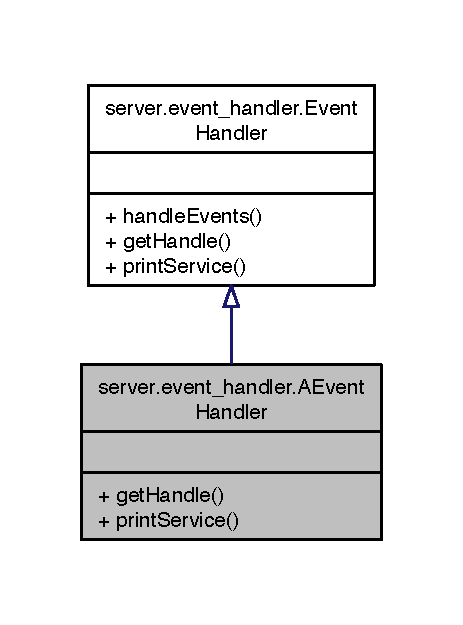
\includegraphics[width=222pt]{classserver_1_1event__handler_1_1_a_event_handler__inherit__graph}
\end{center}
\end{figure}


server.\-event\-\_\-handler.\-A\-Event\-Handler에 대한 협력 다이어그램\-:
\nopagebreak
\begin{figure}[H]
\begin{center}
\leavevmode
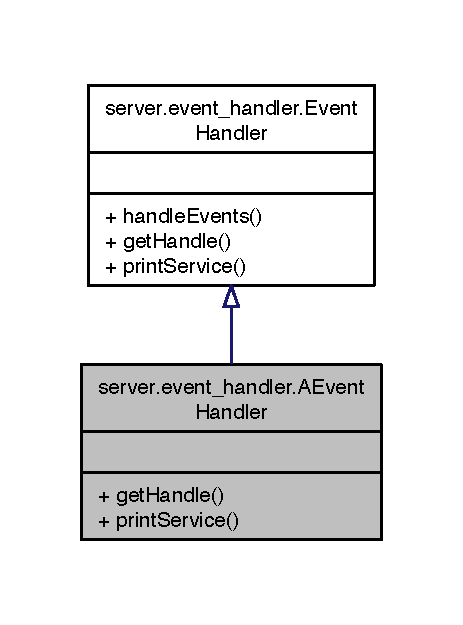
\includegraphics[width=222pt]{classserver_1_1event__handler_1_1_a_event_handler__coll__graph}
\end{center}
\end{figure}
\subsection*{Public 멤버 함수}
\begin{DoxyCompactItemize}
\item 
String \hyperlink{classserver_1_1event__handler_1_1_a_event_handler_a7c98e1d240b5afaf1b4ffbfd18e2f048}{get\-Handle} ()
\item 
void \hyperlink{classserver_1_1event__handler_1_1_a_event_handler_adb8e52f8efa68b7ffcab48962fb50efc}{print\-Service} (String name, String age)
\item 
void \hyperlink{classserver_1_1event__handler_1_1_event_handler_a5d28300da533ce9dad96d26cc0aa8eda}{handle\-Events} (String params)
\end{DoxyCompactItemize}


\subsection{상세한 설명}
A 이벤트 핸들러. 

A\-Event\-Handler.\-java 파일의 6 번째 라인에서 정의되었습니다.



\subsection{멤버 함수 문서화}
\hypertarget{classserver_1_1event__handler_1_1_a_event_handler_a7c98e1d240b5afaf1b4ffbfd18e2f048}{\index{server\-::event\-\_\-handler\-::\-A\-Event\-Handler@{server\-::event\-\_\-handler\-::\-A\-Event\-Handler}!get\-Handle@{get\-Handle}}
\index{get\-Handle@{get\-Handle}!server::event_handler::AEventHandler@{server\-::event\-\_\-handler\-::\-A\-Event\-Handler}}
\subsubsection[{get\-Handle}]{\setlength{\rightskip}{0pt plus 5cm}String server.\-event\-\_\-handler.\-A\-Event\-Handler.\-get\-Handle (
\begin{DoxyParamCaption}
{}
\end{DoxyParamCaption}
)}}\label{classserver_1_1event__handler_1_1_a_event_handler_a7c98e1d240b5afaf1b4ffbfd18e2f048}
A 이벤트 핸들러의 키값을 반환한다. 
\begin{DoxyParams}{매개변수}
{\em @return} & Handle\-Key A 이벤트 핸들러의 키값. \\
\hline
\end{DoxyParams}


A\-Event\-Handler.\-java 파일의 13 번째 라인에서 정의되었습니다.


\begin{DoxyCode}
13                               \{
14         \textcolor{keywordflow}{return} \textcolor{stringliteral}{"0x5001"};
15     \}
\end{DoxyCode}
\hypertarget{classserver_1_1event__handler_1_1_event_handler_a5d28300da533ce9dad96d26cc0aa8eda}{\index{server\-::event\-\_\-handler\-::\-A\-Event\-Handler@{server\-::event\-\_\-handler\-::\-A\-Event\-Handler}!handle\-Events@{handle\-Events}}
\index{handle\-Events@{handle\-Events}!server::event_handler::AEventHandler@{server\-::event\-\_\-handler\-::\-A\-Event\-Handler}}
\subsubsection[{handle\-Events}]{\setlength{\rightskip}{0pt plus 5cm}void server.\-event\-\_\-handler.\-Event\-Handler.\-handle\-Events (
\begin{DoxyParamCaption}
\item[{String}]{params}
\end{DoxyParamCaption}
)\hspace{0.3cm}{\ttfamily [inherited]}}}\label{classserver_1_1event__handler_1_1_event_handler_a5d28300da533ce9dad96d26cc0aa8eda}
핸들러에 전달된 이벤트를 파싱하여 처리한다. 
\begin{DoxyParams}{매개변수}
{\em params} & 핸들러가 파싱하여 처리할 문자열. \\
\hline
\end{DoxyParams}
\begin{DoxyReturn}{반환값}
Nothing 
\end{DoxyReturn}


Event\-Handler.\-java 파일의 14 번째 라인에서 정의되었습니다.


\begin{DoxyCode}
14                                             \{
15         String[] arr = \textcolor{keyword}{new} String[2];
16 
17         StringTokenizer token = \textcolor{keyword}{new} StringTokenizer(params, \textcolor{stringliteral}{"|"});
18         \textcolor{keywordtype}{int} i = 0;
19         \textcolor{keywordflow}{while} (token.hasMoreTokens())
20             arr[i++] = token.nextToken();
21 
22         String str1 = arr[0];
23         String str2 = arr[1];
24 
25         \hyperlink{classserver_1_1event__handler_1_1_event_handler_afc87125b5bd2e5d255a4fd0af12bebcb}{printService}(str1, str2);
26     \}
\end{DoxyCode}


이 함수 내부에서 호출하는 함수들에 대한 그래프입니다.\-:
\nopagebreak
\begin{figure}[H]
\begin{center}
\leavevmode
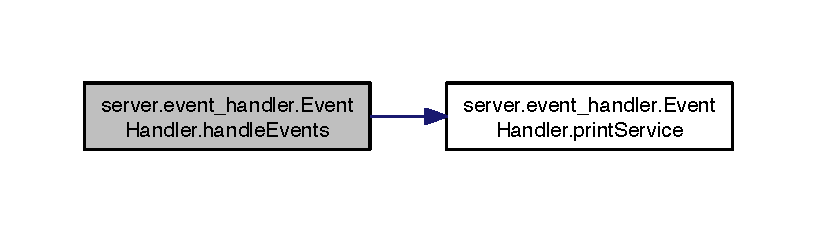
\includegraphics[width=350pt]{classserver_1_1event__handler_1_1_event_handler_a5d28300da533ce9dad96d26cc0aa8eda_cgraph}
\end{center}
\end{figure}


\hypertarget{classserver_1_1event__handler_1_1_a_event_handler_adb8e52f8efa68b7ffcab48962fb50efc}{\index{server\-::event\-\_\-handler\-::\-A\-Event\-Handler@{server\-::event\-\_\-handler\-::\-A\-Event\-Handler}!print\-Service@{print\-Service}}
\index{print\-Service@{print\-Service}!server::event_handler::AEventHandler@{server\-::event\-\_\-handler\-::\-A\-Event\-Handler}}
\subsubsection[{print\-Service}]{\setlength{\rightskip}{0pt plus 5cm}void server.\-event\-\_\-handler.\-A\-Event\-Handler.\-print\-Service (
\begin{DoxyParamCaption}
\item[{String}]{name, }
\item[{String}]{age}
\end{DoxyParamCaption}
)}}\label{classserver_1_1event__handler_1_1_a_event_handler_adb8e52f8efa68b7ffcab48962fb50efc}
A 이벤트를 출력하는 서비스. 
\begin{DoxyParams}{매개변수}
{\em name} & 이름. \\
\hline
{\em age} & 나이. \\
\hline
\end{DoxyParams}
\begin{DoxyReturn}{반환값}
Nothing 
\end{DoxyReturn}


A\-Event\-Handler.\-java 파일의 24 번째 라인에서 정의되었습니다.


\begin{DoxyCode}
24                                                       \{
25         System.out.println(\textcolor{stringliteral}{"A Service print called..."});
26         System.out.println(\textcolor{stringliteral}{"Param -> name :"} + name + \textcolor{stringliteral}{" age : "} + age);
27     \}
\end{DoxyCode}


이 클래스에 대한 문서화 페이지는 다음의 파일로부터 생성되었습니다.\-:\begin{DoxyCompactItemize}
\item 
src/server/event\-\_\-handler/\hyperlink{_a_event_handler_8java}{A\-Event\-Handler.\-java}\end{DoxyCompactItemize}

\hypertarget{classserver_1_1event__handler_1_1_b_event_handler}{\section{server.\-event\-\_\-handler.\-B\-Event\-Handler 클래스 참조}
\label{classserver_1_1event__handler_1_1_b_event_handler}\index{server.\-event\-\_\-handler.\-B\-Event\-Handler@{server.\-event\-\_\-handler.\-B\-Event\-Handler}}
}


server.\-event\-\_\-handler.\-B\-Event\-Handler에 대한 상속 다이어그램 \-: 
\nopagebreak
\begin{figure}[H]
\begin{center}
\leavevmode
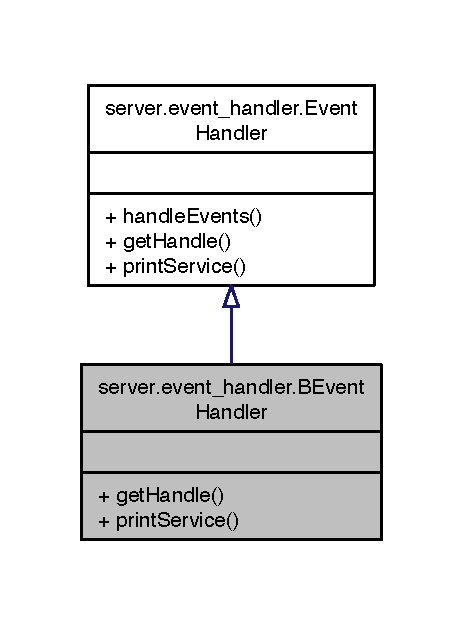
\includegraphics[width=222pt]{classserver_1_1event__handler_1_1_b_event_handler__inherit__graph}
\end{center}
\end{figure}


server.\-event\-\_\-handler.\-B\-Event\-Handler에 대한 협력 다이어그램\-:
\nopagebreak
\begin{figure}[H]
\begin{center}
\leavevmode
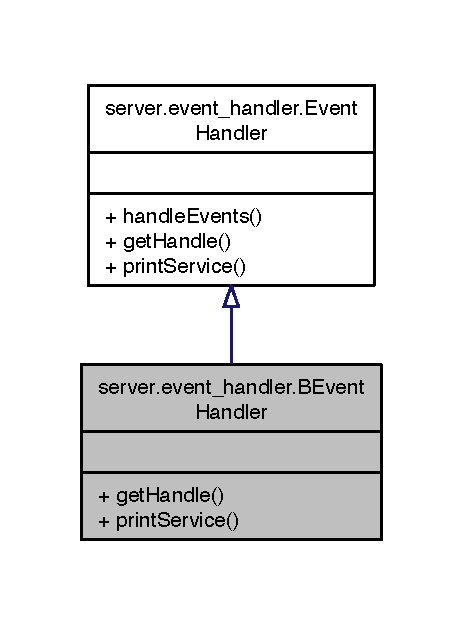
\includegraphics[width=222pt]{classserver_1_1event__handler_1_1_b_event_handler__coll__graph}
\end{center}
\end{figure}
\subsection*{Public 멤버 함수}
\begin{DoxyCompactItemize}
\item 
String \hyperlink{classserver_1_1event__handler_1_1_b_event_handler_a70f6eebfe960f4dd8bf0a3ecad7b0a0e}{get\-Handle} ()
\item 
void \hyperlink{classserver_1_1event__handler_1_1_b_event_handler_a68fcd12b9a8814ef86cb2ede1f9165bb}{print\-Service} (String nation, String city)
\item 
void \hyperlink{classserver_1_1event__handler_1_1_event_handler_a5d28300da533ce9dad96d26cc0aa8eda}{handle\-Events} (String params)
\end{DoxyCompactItemize}


\subsection{상세한 설명}
B 이벤트 핸들러. 

B\-Event\-Handler.\-java 파일의 6 번째 라인에서 정의되었습니다.



\subsection{멤버 함수 문서화}
\hypertarget{classserver_1_1event__handler_1_1_b_event_handler_a70f6eebfe960f4dd8bf0a3ecad7b0a0e}{\index{server\-::event\-\_\-handler\-::\-B\-Event\-Handler@{server\-::event\-\_\-handler\-::\-B\-Event\-Handler}!get\-Handle@{get\-Handle}}
\index{get\-Handle@{get\-Handle}!server::event_handler::BEventHandler@{server\-::event\-\_\-handler\-::\-B\-Event\-Handler}}
\subsubsection[{get\-Handle}]{\setlength{\rightskip}{0pt plus 5cm}String server.\-event\-\_\-handler.\-B\-Event\-Handler.\-get\-Handle (
\begin{DoxyParamCaption}
{}
\end{DoxyParamCaption}
)}}\label{classserver_1_1event__handler_1_1_b_event_handler_a70f6eebfe960f4dd8bf0a3ecad7b0a0e}
B 이벤트 핸들러의 키값을 반환한다. 
\begin{DoxyParams}{매개변수}
{\em @return} & Handle\-Key B 이벤트 핸들러의 키값. \\
\hline
\end{DoxyParams}


B\-Event\-Handler.\-java 파일의 13 번째 라인에서 정의되었습니다.


\begin{DoxyCode}
13                               \{
14         \textcolor{keywordflow}{return} \textcolor{stringliteral}{"0x6001"};
15     \}
\end{DoxyCode}
\hypertarget{classserver_1_1event__handler_1_1_event_handler_a5d28300da533ce9dad96d26cc0aa8eda}{\index{server\-::event\-\_\-handler\-::\-B\-Event\-Handler@{server\-::event\-\_\-handler\-::\-B\-Event\-Handler}!handle\-Events@{handle\-Events}}
\index{handle\-Events@{handle\-Events}!server::event_handler::BEventHandler@{server\-::event\-\_\-handler\-::\-B\-Event\-Handler}}
\subsubsection[{handle\-Events}]{\setlength{\rightskip}{0pt plus 5cm}void server.\-event\-\_\-handler.\-Event\-Handler.\-handle\-Events (
\begin{DoxyParamCaption}
\item[{String}]{params}
\end{DoxyParamCaption}
)\hspace{0.3cm}{\ttfamily [inherited]}}}\label{classserver_1_1event__handler_1_1_event_handler_a5d28300da533ce9dad96d26cc0aa8eda}
핸들러에 전달된 이벤트를 파싱하여 처리한다. 
\begin{DoxyParams}{매개변수}
{\em params} & 핸들러가 파싱하여 처리할 문자열. \\
\hline
\end{DoxyParams}
\begin{DoxyReturn}{반환값}
Nothing 
\end{DoxyReturn}


Event\-Handler.\-java 파일의 14 번째 라인에서 정의되었습니다.


\begin{DoxyCode}
14                                             \{
15         String[] arr = \textcolor{keyword}{new} String[2];
16 
17         StringTokenizer token = \textcolor{keyword}{new} StringTokenizer(params, \textcolor{stringliteral}{"|"});
18         \textcolor{keywordtype}{int} i = 0;
19         \textcolor{keywordflow}{while} (token.hasMoreTokens())
20             arr[i++] = token.nextToken();
21 
22         String str1 = arr[0];
23         String str2 = arr[1];
24 
25         \hyperlink{classserver_1_1event__handler_1_1_event_handler_afc87125b5bd2e5d255a4fd0af12bebcb}{printService}(str1, str2);
26     \}
\end{DoxyCode}


이 함수 내부에서 호출하는 함수들에 대한 그래프입니다.\-:
\nopagebreak
\begin{figure}[H]
\begin{center}
\leavevmode
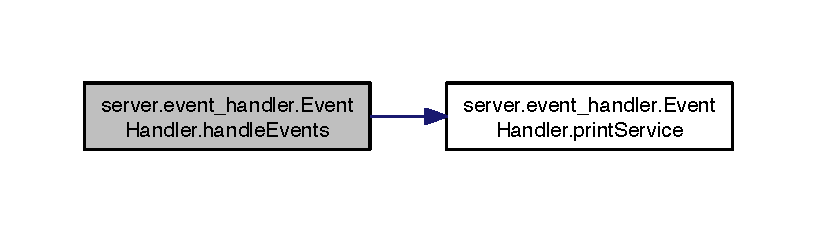
\includegraphics[width=350pt]{classserver_1_1event__handler_1_1_event_handler_a5d28300da533ce9dad96d26cc0aa8eda_cgraph}
\end{center}
\end{figure}


\hypertarget{classserver_1_1event__handler_1_1_b_event_handler_a68fcd12b9a8814ef86cb2ede1f9165bb}{\index{server\-::event\-\_\-handler\-::\-B\-Event\-Handler@{server\-::event\-\_\-handler\-::\-B\-Event\-Handler}!print\-Service@{print\-Service}}
\index{print\-Service@{print\-Service}!server::event_handler::BEventHandler@{server\-::event\-\_\-handler\-::\-B\-Event\-Handler}}
\subsubsection[{print\-Service}]{\setlength{\rightskip}{0pt plus 5cm}void server.\-event\-\_\-handler.\-B\-Event\-Handler.\-print\-Service (
\begin{DoxyParamCaption}
\item[{String}]{nation, }
\item[{String}]{city}
\end{DoxyParamCaption}
)}}\label{classserver_1_1event__handler_1_1_b_event_handler_a68fcd12b9a8814ef86cb2ede1f9165bb}
B 이벤트를 출력하는 서비스. 
\begin{DoxyParams}{매개변수}
{\em nation} & 나라. \\
\hline
{\em city} & 도시. \\
\hline
\end{DoxyParams}
\begin{DoxyReturn}{반환값}
Nothing 
\end{DoxyReturn}


B\-Event\-Handler.\-java 파일의 24 번째 라인에서 정의되었습니다.


\begin{DoxyCode}
24                                                          \{
25         System.out.println(\textcolor{stringliteral}{"B Service print called..."});
26         System.out.println(\textcolor{stringliteral}{"Param -> nation :"} + nation + \textcolor{stringliteral}{" city : "} + city);
27     \}
\end{DoxyCode}


이 클래스에 대한 문서화 페이지는 다음의 파일로부터 생성되었습니다.\-:\begin{DoxyCompactItemize}
\item 
src/server/event\-\_\-handler/\hyperlink{_b_event_handler_8java}{B\-Event\-Handler.\-java}\end{DoxyCompactItemize}

\hypertarget{classserver_1_1_demultiplexer}{\section{server.\-Demultiplexer 클래스 참조}
\label{classserver_1_1_demultiplexer}\index{server.\-Demultiplexer@{server.\-Demultiplexer}}
}


이벤트를 디코딩하여 적절한 핸들러에 전달한다.  




server.\-Demultiplexer에 대한 협력 다이어그램\-:\nopagebreak
\begin{figure}[H]
\begin{center}
\leavevmode
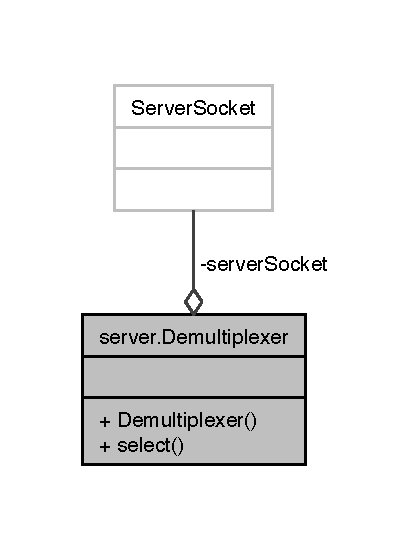
\includegraphics[width=197pt]{classserver_1_1_demultiplexer__coll__graph}
\end{center}
\end{figure}
\subsection*{Public 멤버 함수}
\begin{DoxyCompactItemize}
\item 
\hyperlink{classserver_1_1_demultiplexer_a29f6adc4249c7e6603c84821ba994159}{Demultiplexer} ()  throws I\-O\-Exception 
\begin{DoxyCompactList}\small\item\em 생성자. \end{DoxyCompactList}\item 
void \hyperlink{classserver_1_1_demultiplexer_ac73b7d090155c7ef0112ea3718162a13}{select} (\hyperlink{classserver_1_1_handle_map}{Handle\-Map} handlers)  throws I\-O\-Exception 
\begin{DoxyCompactList}\small\item\em 이벤트 발생시 Demultiplex 한다. \end{DoxyCompactList}\end{DoxyCompactItemize}
\subsection*{Private 속성}
\begin{DoxyCompactItemize}
\item 
Server\-Socket \hyperlink{classserver_1_1_demultiplexer_a45a45c637b717c6d3114e8f3ade5b477}{server\-Socket}
\item 
final int \hyperlink{classserver_1_1_demultiplexer_aea070faa805aef528fe606091b2d25b2}{H\-E\-A\-D\-E\-R\-\_\-\-S\-I\-Z\-E} = 6
\end{DoxyCompactItemize}


\subsection{상세한 설명}
이벤트를 디코딩하여 적절한 핸들러에 전달한다. 

이벤트가 발생하면 header와 data 부분으로 나눈다. 이중 header는 적절한 handler를 찾는데 쓰이고, data는 handler에 전달한다. 

Demultiplexer.\-java 파일의 12 번째 라인에서 정의되었습니다.



\subsection{생성자 \& 소멸자 문서화}
\hypertarget{classserver_1_1_demultiplexer_a29f6adc4249c7e6603c84821ba994159}{\index{server\-::\-Demultiplexer@{server\-::\-Demultiplexer}!Demultiplexer@{Demultiplexer}}
\index{Demultiplexer@{Demultiplexer}!server::Demultiplexer@{server\-::\-Demultiplexer}}
\subsubsection[{Demultiplexer}]{\setlength{\rightskip}{0pt plus 5cm}server.\-Demultiplexer.\-Demultiplexer (
\begin{DoxyParamCaption}
{}
\end{DoxyParamCaption}
) throws I\-O\-Exception}}\label{classserver_1_1_demultiplexer_a29f6adc4249c7e6603c84821ba994159}


생성자. 

서버 소켓을 생성한다. \begin{DoxyReturn}{반환값}
Nothing 
\end{DoxyReturn}

\begin{DoxyExceptions}{예외}
{\em I\-O\-Exception} & I\-O\-Exception 발생시 던진다. \\
\hline
\end{DoxyExceptions}


Demultiplexer.\-java 파일의 22 번째 라인에서 정의되었습니다.


\begin{DoxyCode}
22                                               \{
23         \hyperlink{classserver_1_1_demultiplexer_a45a45c637b717c6d3114e8f3ade5b477}{serverSocket} = \textcolor{keyword}{new} ServerSocket(5000);
24     \}
\end{DoxyCode}


\subsection{멤버 함수 문서화}
\hypertarget{classserver_1_1_demultiplexer_ac73b7d090155c7ef0112ea3718162a13}{\index{server\-::\-Demultiplexer@{server\-::\-Demultiplexer}!select@{select}}
\index{select@{select}!server::Demultiplexer@{server\-::\-Demultiplexer}}
\subsubsection[{select}]{\setlength{\rightskip}{0pt plus 5cm}void server.\-Demultiplexer.\-select (
\begin{DoxyParamCaption}
\item[{{\bf Handle\-Map}}]{handlers}
\end{DoxyParamCaption}
) throws I\-O\-Exception}}\label{classserver_1_1_demultiplexer_ac73b7d090155c7ef0112ea3718162a13}


이벤트 발생시 Demultiplex 한다. 

이벤트 발생시, header와 data로 나눈다. 이중 header는 적절한 handler를 찾는데 쓰이고, data는 handler에 전달한다. 
\begin{DoxyParams}{매개변수}
{\em handlers} & Reactor에 등록된 핸들맵 객체. \\
\hline
\end{DoxyParams}
\begin{DoxyReturn}{반환값}
Nothing 
\end{DoxyReturn}

\begin{DoxyExceptions}{예외}
{\em I\-O\-Exception} & I\-O\-Exception 발생시 던진다. \\
\hline
\end{DoxyExceptions}


Demultiplexer.\-java 파일의 33 번째 라인에서 정의되었습니다.


\begin{DoxyCode}
33                                                               \{
34         Socket socket = serverSocket.accept();
35         InputStream inputStream = socket.getInputStream();
36 
37         byte[] buffer = \textcolor{keyword}{new} byte[\hyperlink{classserver_1_1_demultiplexer_aea070faa805aef528fe606091b2d25b2}{HEADER\_SIZE}];
38         inputStream.read(buffer);
39         String header = \textcolor{keyword}{new} String(buffer);
40 
41         handlers.get(header).handleEvent(inputStream);
42     \}
\end{DoxyCode}


\subsection{멤버 데이타 문서화}
\hypertarget{classserver_1_1_demultiplexer_aea070faa805aef528fe606091b2d25b2}{\index{server\-::\-Demultiplexer@{server\-::\-Demultiplexer}!H\-E\-A\-D\-E\-R\-\_\-\-S\-I\-Z\-E@{H\-E\-A\-D\-E\-R\-\_\-\-S\-I\-Z\-E}}
\index{H\-E\-A\-D\-E\-R\-\_\-\-S\-I\-Z\-E@{H\-E\-A\-D\-E\-R\-\_\-\-S\-I\-Z\-E}!server::Demultiplexer@{server\-::\-Demultiplexer}}
\subsubsection[{H\-E\-A\-D\-E\-R\-\_\-\-S\-I\-Z\-E}]{\setlength{\rightskip}{0pt plus 5cm}final int server.\-Demultiplexer.\-H\-E\-A\-D\-E\-R\-\_\-\-S\-I\-Z\-E = 6\hspace{0.3cm}{\ttfamily [private]}}}\label{classserver_1_1_demultiplexer_aea070faa805aef528fe606091b2d25b2}


Demultiplexer.\-java 파일의 14 번째 라인에서 정의되었습니다.

\hypertarget{classserver_1_1_demultiplexer_a45a45c637b717c6d3114e8f3ade5b477}{\index{server\-::\-Demultiplexer@{server\-::\-Demultiplexer}!server\-Socket@{server\-Socket}}
\index{server\-Socket@{server\-Socket}!server::Demultiplexer@{server\-::\-Demultiplexer}}
\subsubsection[{server\-Socket}]{\setlength{\rightskip}{0pt plus 5cm}Server\-Socket server.\-Demultiplexer.\-server\-Socket\hspace{0.3cm}{\ttfamily [private]}}}\label{classserver_1_1_demultiplexer_a45a45c637b717c6d3114e8f3ade5b477}


Demultiplexer.\-java 파일의 13 번째 라인에서 정의되었습니다.



이 클래스에 대한 문서화 페이지는 다음의 파일로부터 생성되었습니다.\-:\begin{DoxyCompactItemize}
\item 
src/server/\hyperlink{_demultiplexer_8java}{Demultiplexer.\-java}\end{DoxyCompactItemize}

\hypertarget{classserver_1_1event__handler_1_1_event_handler}{\section{server.\-event\-\_\-handler.\-Event\-Handler 클래스 참조}
\label{classserver_1_1event__handler_1_1_event_handler}\index{server.\-event\-\_\-handler.\-Event\-Handler@{server.\-event\-\_\-handler.\-Event\-Handler}}
}


server.\-event\-\_\-handler.\-Event\-Handler에 대한 상속 다이어그램 \-: 
\nopagebreak
\begin{figure}[H]
\begin{center}
\leavevmode
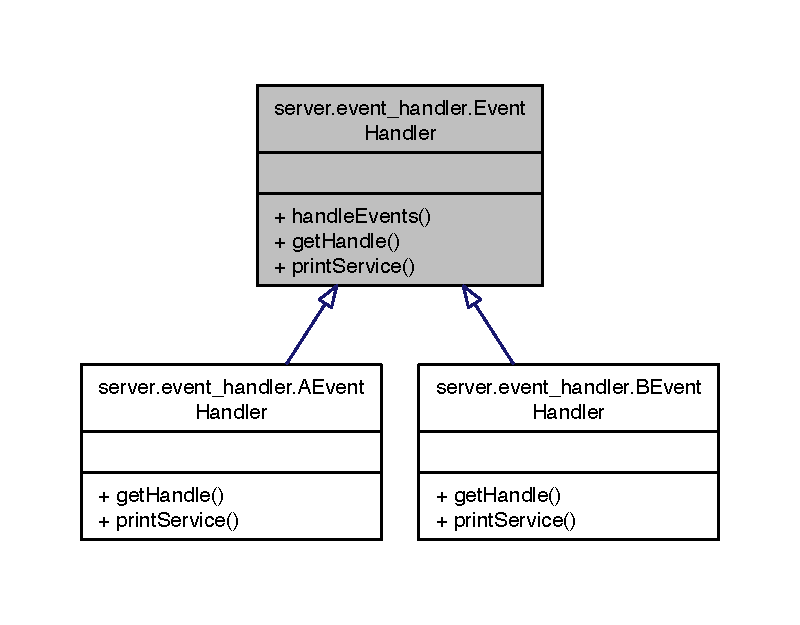
\includegraphics[width=350pt]{classserver_1_1event__handler_1_1_event_handler__inherit__graph}
\end{center}
\end{figure}


server.\-event\-\_\-handler.\-Event\-Handler에 대한 협력 다이어그램\-:
\nopagebreak
\begin{figure}[H]
\begin{center}
\leavevmode
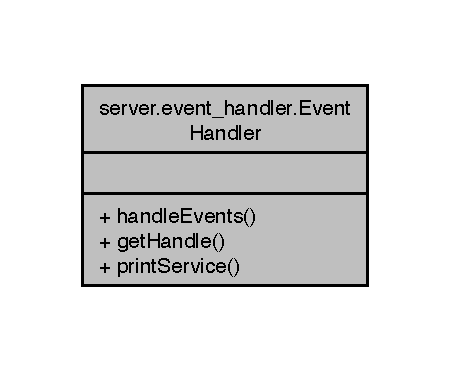
\includegraphics[width=216pt]{classserver_1_1event__handler_1_1_event_handler__coll__graph}
\end{center}
\end{figure}
\subsection*{Public 멤버 함수}
\begin{DoxyCompactItemize}
\item 
void \hyperlink{classserver_1_1event__handler_1_1_event_handler_a5d28300da533ce9dad96d26cc0aa8eda}{handle\-Events} (String params)
\item 
abstract String \hyperlink{classserver_1_1event__handler_1_1_event_handler_a11ebb67c402f4ce26cd18c3a0217f169}{get\-Handle} ()
\item 
abstract void \hyperlink{classserver_1_1event__handler_1_1_event_handler_afc87125b5bd2e5d255a4fd0af12bebcb}{print\-Service} (String str1, String str2)
\end{DoxyCompactItemize}


\subsection{상세한 설명}
이벤트 핸들러를 정의하는 추상클래스. 

Event\-Handler.\-java 파일의 8 번째 라인에서 정의되었습니다.



\subsection{멤버 함수 문서화}
\hypertarget{classserver_1_1event__handler_1_1_event_handler_a11ebb67c402f4ce26cd18c3a0217f169}{\index{server\-::event\-\_\-handler\-::\-Event\-Handler@{server\-::event\-\_\-handler\-::\-Event\-Handler}!get\-Handle@{get\-Handle}}
\index{get\-Handle@{get\-Handle}!server::event_handler::EventHandler@{server\-::event\-\_\-handler\-::\-Event\-Handler}}
\subsubsection[{get\-Handle}]{\setlength{\rightskip}{0pt plus 5cm}abstract String server.\-event\-\_\-handler.\-Event\-Handler.\-get\-Handle (
\begin{DoxyParamCaption}
{}
\end{DoxyParamCaption}
)\hspace{0.3cm}{\ttfamily [abstract]}}}\label{classserver_1_1event__handler_1_1_event_handler_a11ebb67c402f4ce26cd18c3a0217f169}
특정 이벤트 핸들러의 키값을 반환하는 추상메서드. 
\begin{DoxyParams}{매개변수}
{\em @return} & Handle\-Key 특정 이벤트 핸들러의 키값 \\
\hline
\end{DoxyParams}
\hypertarget{classserver_1_1event__handler_1_1_event_handler_a5d28300da533ce9dad96d26cc0aa8eda}{\index{server\-::event\-\_\-handler\-::\-Event\-Handler@{server\-::event\-\_\-handler\-::\-Event\-Handler}!handle\-Events@{handle\-Events}}
\index{handle\-Events@{handle\-Events}!server::event_handler::EventHandler@{server\-::event\-\_\-handler\-::\-Event\-Handler}}
\subsubsection[{handle\-Events}]{\setlength{\rightskip}{0pt plus 5cm}void server.\-event\-\_\-handler.\-Event\-Handler.\-handle\-Events (
\begin{DoxyParamCaption}
\item[{String}]{params}
\end{DoxyParamCaption}
)}}\label{classserver_1_1event__handler_1_1_event_handler_a5d28300da533ce9dad96d26cc0aa8eda}
핸들러에 전달된 이벤트를 파싱하여 처리한다. 
\begin{DoxyParams}{매개변수}
{\em params} & 핸들러가 파싱하여 처리할 문자열. \\
\hline
\end{DoxyParams}
\begin{DoxyReturn}{반환값}
Nothing 
\end{DoxyReturn}


Event\-Handler.\-java 파일의 14 번째 라인에서 정의되었습니다.


\begin{DoxyCode}
14                                             \{
15         String[] arr = \textcolor{keyword}{new} String[2];
16 
17         StringTokenizer token = \textcolor{keyword}{new} StringTokenizer(params, \textcolor{stringliteral}{"|"});
18         \textcolor{keywordtype}{int} i = 0;
19         \textcolor{keywordflow}{while} (token.hasMoreTokens())
20             arr[i++] = token.nextToken();
21 
22         String str1 = arr[0];
23         String str2 = arr[1];
24 
25         \hyperlink{classserver_1_1event__handler_1_1_event_handler_afc87125b5bd2e5d255a4fd0af12bebcb}{printService}(str1, str2);
26     \}
\end{DoxyCode}


이 함수 내부에서 호출하는 함수들에 대한 그래프입니다.\-:
\nopagebreak
\begin{figure}[H]
\begin{center}
\leavevmode
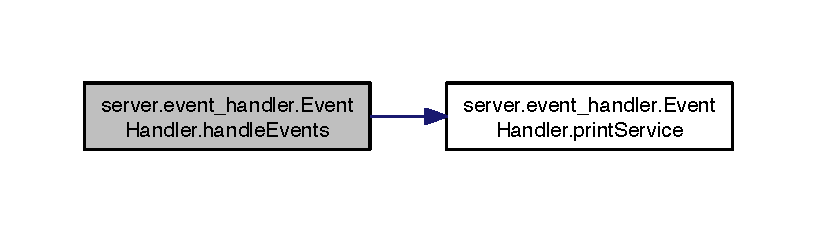
\includegraphics[width=350pt]{classserver_1_1event__handler_1_1_event_handler_a5d28300da533ce9dad96d26cc0aa8eda_cgraph}
\end{center}
\end{figure}


\hypertarget{classserver_1_1event__handler_1_1_event_handler_afc87125b5bd2e5d255a4fd0af12bebcb}{\index{server\-::event\-\_\-handler\-::\-Event\-Handler@{server\-::event\-\_\-handler\-::\-Event\-Handler}!print\-Service@{print\-Service}}
\index{print\-Service@{print\-Service}!server::event_handler::EventHandler@{server\-::event\-\_\-handler\-::\-Event\-Handler}}
\subsubsection[{print\-Service}]{\setlength{\rightskip}{0pt plus 5cm}abstract void server.\-event\-\_\-handler.\-Event\-Handler.\-print\-Service (
\begin{DoxyParamCaption}
\item[{String}]{str1, }
\item[{String}]{str2}
\end{DoxyParamCaption}
)\hspace{0.3cm}{\ttfamily [abstract]}}}\label{classserver_1_1event__handler_1_1_event_handler_afc87125b5bd2e5d255a4fd0af12bebcb}
특정 이벤트를 출력하는 콜백메서드. 
\begin{DoxyParams}{매개변수}
{\em str1} & 출력할 문자열 객체1 \\
\hline
{\em str2} & 출력할 문자열 객체2 \\
\hline
\end{DoxyParams}
\begin{DoxyReturn}{반환값}
Nothing 
\end{DoxyReturn}


이 함수를 호출하는 함수들에 대한 그래프입니다.\-:
\nopagebreak
\begin{figure}[H]
\begin{center}
\leavevmode
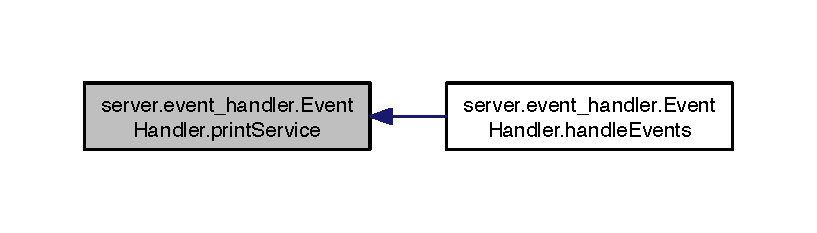
\includegraphics[width=350pt]{classserver_1_1event__handler_1_1_event_handler_afc87125b5bd2e5d255a4fd0af12bebcb_icgraph}
\end{center}
\end{figure}




이 클래스에 대한 문서화 페이지는 다음의 파일로부터 생성되었습니다.\-:\begin{DoxyCompactItemize}
\item 
src/server/event\-\_\-handler/\hyperlink{_event_handler_8java}{Event\-Handler.\-java}\end{DoxyCompactItemize}

\hypertarget{classserver_1_1_handle_map}{\section{server.\-Handle\-Map 클래스 참조}
\label{classserver_1_1_handle_map}\index{server.\-Handle\-Map@{server.\-Handle\-Map}}
}


server.\-Handle\-Map에 대한 상속 다이어그램 \-: 
\nopagebreak
\begin{figure}[H]
\begin{center}
\leavevmode
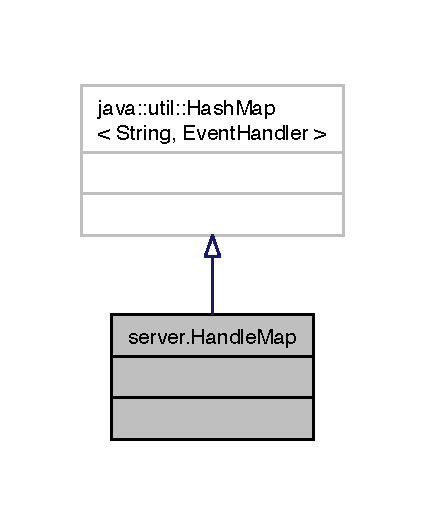
\includegraphics[width=204pt]{classserver_1_1_handle_map__inherit__graph}
\end{center}
\end{figure}


server.\-Handle\-Map에 대한 협력 다이어그램\-:
\nopagebreak
\begin{figure}[H]
\begin{center}
\leavevmode
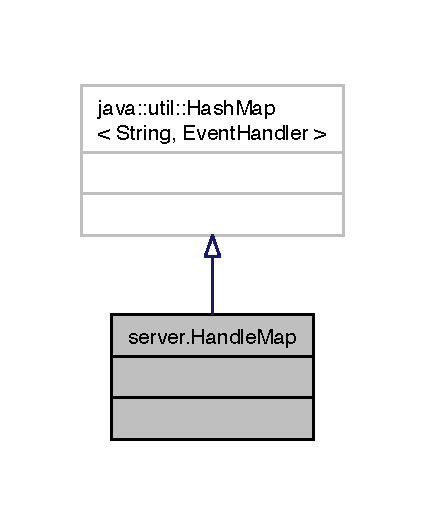
\includegraphics[width=204pt]{classserver_1_1_handle_map__coll__graph}
\end{center}
\end{figure}


\subsection{상세한 설명}
핸들과 이벤트 핸들러를 해쉬 형태로 저장하는 객체. 

Handle\-Map.\-java 파일의 10 번째 라인에서 정의되었습니다.



이 클래스에 대한 문서화 페이지는 다음의 파일로부터 생성되었습니다.\-:\begin{DoxyCompactItemize}
\item 
src/server/\hyperlink{_handle_map_8java}{Handle\-Map.\-java}\end{DoxyCompactItemize}

\hypertarget{classclient_1_1_main}{\section{client.\-Main 클래스 참조}
\label{classclient_1_1_main}\index{client.\-Main@{client.\-Main}}
}


client.\-Main에 대한 협력 다이어그램\-:
\nopagebreak
\begin{figure}[H]
\begin{center}
\leavevmode
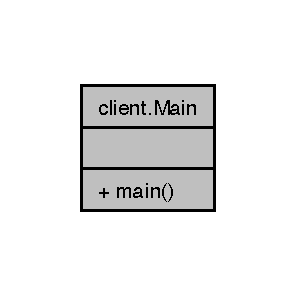
\includegraphics[width=142pt]{classclient_1_1_main__coll__graph}
\end{center}
\end{figure}
\subsection*{정적 Public 멤버 함수}
\begin{DoxyCompactItemize}
\item 
static void \hyperlink{classclient_1_1_main_a757d493b68aa66d3d3c2e71a1c6e4c0e}{main} (String\mbox{[}$\,$\mbox{]} args)  throws Unknown\-Host\-Exception, I\-O\-Exception, Interrupted\-Exception 
\end{DoxyCompactItemize}


\subsection{상세한 설명}


Main.\-java 파일의 8 번째 라인에서 정의되었습니다.



\subsection{멤버 함수 문서화}
\hypertarget{classclient_1_1_main_a757d493b68aa66d3d3c2e71a1c6e4c0e}{\index{client\-::\-Main@{client\-::\-Main}!main@{main}}
\index{main@{main}!client::Main@{client\-::\-Main}}
\subsubsection[{main}]{\setlength{\rightskip}{0pt plus 5cm}static void client.\-Main.\-main (
\begin{DoxyParamCaption}
\item[{String\mbox{[}$\,$\mbox{]}}]{args}
\end{DoxyParamCaption}
) throws Unknown\-Host\-Exception, I\-O\-Exception, Interrupted\-Exception\hspace{0.3cm}{\ttfamily [static]}}}\label{classclient_1_1_main_a757d493b68aa66d3d3c2e71a1c6e4c0e}


Main.\-java 파일의 10 번째 라인에서 정의되었습니다.


\begin{DoxyCode}
10                                                                                                           \{
11         \textcolor{keywordflow}{while} (\textcolor{keyword}{true}) \{
12             \{
13                 Socket socket = \textcolor{keyword}{new} Socket(\textcolor{stringliteral}{"127.0.0.1"}, 5000);
14                 OutputStream out = socket.getOutputStream();
15                 out.write(\textcolor{stringliteral}{"0x5001|김동국|21"}.getBytes());
16                 socket.close();
17             \}
18             \{
19                 Socket socket = \textcolor{keyword}{new} Socket(\textcolor{stringliteral}{"127.0.0.1"}, 5000);
20                 OutputStream out = socket.getOutputStream();
21                 out.write(\textcolor{stringliteral}{"0x6001|대한민국|서울"}.getBytes());
22                 socket.close();
23             \}
24             Thread.sleep(1000);
25         \}
26     \}
\end{DoxyCode}


이 클래스에 대한 문서화 페이지는 다음의 파일로부터 생성되었습니다.\-:\begin{DoxyCompactItemize}
\item 
src/client/\hyperlink{_main_8java}{Main.\-java}\end{DoxyCompactItemize}

\hypertarget{classserver_1_1_reactor}{\section{server.\-Reactor 클래스 참조}
\label{classserver_1_1_reactor}\index{server.\-Reactor@{server.\-Reactor}}
}


server.\-Reactor에 대한 협력 다이어그램\-:
\nopagebreak
\begin{figure}[H]
\begin{center}
\leavevmode
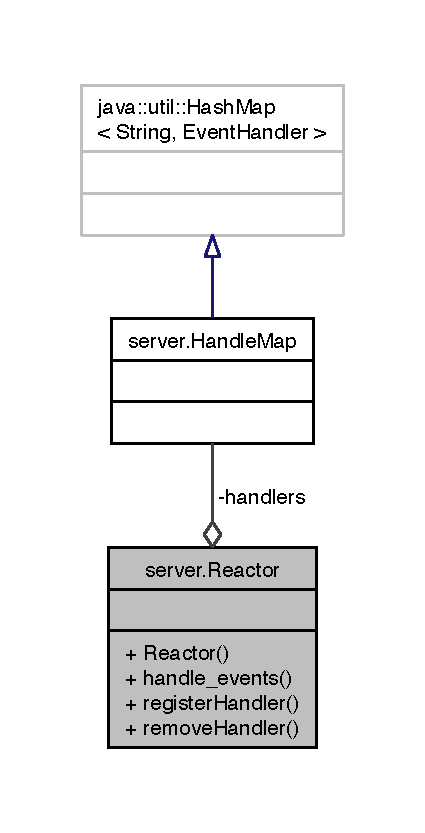
\includegraphics[width=204pt]{classserver_1_1_reactor__coll__graph}
\end{center}
\end{figure}
\subsection*{Public 멤버 함수}
\begin{DoxyCompactItemize}
\item 
\hyperlink{classserver_1_1_reactor_ad32bfcaec7e42dfd6aab98c462af98cf}{Reactor} ()
\item 
void \hyperlink{classserver_1_1_reactor_a6049200905b17b4aba0de79b6df0f5d2}{handle\-\_\-events} ()  throws I\-O\-Exception 
\item 
void \hyperlink{classserver_1_1_reactor_a3e668edae20fadfc4063a83a74001fda}{register\-Handler} (\hyperlink{classserver_1_1event__handler_1_1_event_handler}{Event\-Handler} handler)
\item 
void \hyperlink{classserver_1_1_reactor_a936c855c6581047687a117c0ee76a296}{remove\-Handler} (\hyperlink{classserver_1_1event__handler_1_1_event_handler}{Event\-Handler} handler)
\end{DoxyCompactItemize}
\subsection*{Private 속성}
\begin{DoxyCompactItemize}
\item 
\hyperlink{classserver_1_1_handle_map}{Handle\-Map} \hyperlink{classserver_1_1_reactor_a68f3383c5eb092e372bcf4f39015334f}{handlers}
\end{DoxyCompactItemize}


\subsection{상세한 설명}
이벤트 핸들러를 관리하는 객체. 

Reactor.\-java 파일의 10 번째 라인에서 정의되었습니다.



\subsection{생성자 \& 소멸자 문서화}
\hypertarget{classserver_1_1_reactor_ad32bfcaec7e42dfd6aab98c462af98cf}{\index{server\-::\-Reactor@{server\-::\-Reactor}!Reactor@{Reactor}}
\index{Reactor@{Reactor}!server::Reactor@{server\-::\-Reactor}}
\subsubsection[{Reactor}]{\setlength{\rightskip}{0pt plus 5cm}server.\-Reactor.\-Reactor (
\begin{DoxyParamCaption}
{}
\end{DoxyParamCaption}
)}}\label{classserver_1_1_reactor_ad32bfcaec7e42dfd6aab98c462af98cf}
\hyperlink{classserver_1_1_reactor}{Reactor} 생성자. 핸들과 이벤트 핸들러를 관리할 핸들맵을 초기화한다. 
\begin{DoxyParams}{매개변수}
{\em @return} & Nothing \\
\hline
\end{DoxyParams}


Reactor.\-java 파일의 18 번째 라인에서 정의되었습니다.


\begin{DoxyCode}
18                      \{
19         \hyperlink{classserver_1_1_reactor_a68f3383c5eb092e372bcf4f39015334f}{handlers} = \textcolor{keyword}{new} HandleMap();
20     \}
\end{DoxyCode}


\subsection{멤버 함수 문서화}
\hypertarget{classserver_1_1_reactor_a6049200905b17b4aba0de79b6df0f5d2}{\index{server\-::\-Reactor@{server\-::\-Reactor}!handle\-\_\-events@{handle\-\_\-events}}
\index{handle\-\_\-events@{handle\-\_\-events}!server::Reactor@{server\-::\-Reactor}}
\subsubsection[{handle\-\_\-events}]{\setlength{\rightskip}{0pt plus 5cm}void server.\-Reactor.\-handle\-\_\-events (
\begin{DoxyParamCaption}
{}
\end{DoxyParamCaption}
) throws I\-O\-Exception}}\label{classserver_1_1_reactor_a6049200905b17b4aba0de79b6df0f5d2}
디멀티플렉서에 select 명령을 한다. 
\begin{DoxyParams}{매개변수}
{\em @throws} & I\-O\-Exception \\
\hline
\end{DoxyParams}
\begin{DoxyReturn}{반환값}
Nothing 
\end{DoxyReturn}


Reactor.\-java 파일의 28 번째 라인에서 정의되었습니다.


\begin{DoxyCode}
28                                                    \{
29         Demultiplexer demultiplexer = \textcolor{keyword}{new} Demultiplexer();
30         \textcolor{keywordflow}{while} (\textcolor{keyword}{true}) \{
31             demultiplexer.select(\hyperlink{classserver_1_1_reactor_a68f3383c5eb092e372bcf4f39015334f}{handlers});
32         \}
33     \}
\end{DoxyCode}
\hypertarget{classserver_1_1_reactor_a3e668edae20fadfc4063a83a74001fda}{\index{server\-::\-Reactor@{server\-::\-Reactor}!register\-Handler@{register\-Handler}}
\index{register\-Handler@{register\-Handler}!server::Reactor@{server\-::\-Reactor}}
\subsubsection[{register\-Handler}]{\setlength{\rightskip}{0pt plus 5cm}void server.\-Reactor.\-register\-Handler (
\begin{DoxyParamCaption}
\item[{{\bf Event\-Handler}}]{handler}
\end{DoxyParamCaption}
)}}\label{classserver_1_1_reactor_a3e668edae20fadfc4063a83a74001fda}
Reactor에 이벤트 핸들러를 등록한다. 
\begin{DoxyParams}{매개변수}
{\em handler} & 특정 이벤트를 처리할 핸들러 \\
\hline
\end{DoxyParams}
\begin{DoxyReturn}{반환값}
Nothing 
\end{DoxyReturn}


Reactor.\-java 파일의 40 번째 라인에서 정의되었습니다.


\begin{DoxyCode}
40                                                       \{
41         handlers.put(handler.getHandle(), handler);
42     \}
\end{DoxyCode}
\hypertarget{classserver_1_1_reactor_a936c855c6581047687a117c0ee76a296}{\index{server\-::\-Reactor@{server\-::\-Reactor}!remove\-Handler@{remove\-Handler}}
\index{remove\-Handler@{remove\-Handler}!server::Reactor@{server\-::\-Reactor}}
\subsubsection[{remove\-Handler}]{\setlength{\rightskip}{0pt plus 5cm}void server.\-Reactor.\-remove\-Handler (
\begin{DoxyParamCaption}
\item[{{\bf Event\-Handler}}]{handler}
\end{DoxyParamCaption}
)}}\label{classserver_1_1_reactor_a936c855c6581047687a117c0ee76a296}
Reactor에 이벤트 핸들러를 제거한다. 
\begin{DoxyParams}{매개변수}
{\em handler} & 특정 이벤트를 처리할 핸들러 \\
\hline
\end{DoxyParams}
\begin{DoxyReturn}{반환값}
Nothing 
\end{DoxyReturn}


Reactor.\-java 파일의 49 번째 라인에서 정의되었습니다.


\begin{DoxyCode}
49                                                     \{
50         handlers.remove(handler.getHandle());
51     \}
\end{DoxyCode}


\subsection{멤버 데이타 문서화}
\hypertarget{classserver_1_1_reactor_a68f3383c5eb092e372bcf4f39015334f}{\index{server\-::\-Reactor@{server\-::\-Reactor}!handlers@{handlers}}
\index{handlers@{handlers}!server::Reactor@{server\-::\-Reactor}}
\subsubsection[{handlers}]{\setlength{\rightskip}{0pt plus 5cm}{\bf Handle\-Map} server.\-Reactor.\-handlers\hspace{0.3cm}{\ttfamily [private]}}}\label{classserver_1_1_reactor_a68f3383c5eb092e372bcf4f39015334f}


Reactor.\-java 파일의 11 번째 라인에서 정의되었습니다.



이 클래스에 대한 문서화 페이지는 다음의 파일로부터 생성되었습니다.\-:\begin{DoxyCompactItemize}
\item 
src/server/\hyperlink{_reactor_8java}{Reactor.\-java}\end{DoxyCompactItemize}

\hypertarget{classserver_1_1_server_initialize}{\section{server.\-Server\-Initialize 클래스 참조}
\label{classserver_1_1_server_initialize}\index{server.\-Server\-Initialize@{server.\-Server\-Initialize}}
}


서버 초기화 클래스  




server.\-Server\-Initialize에 대한 협력 다이어그램\-:\nopagebreak
\begin{figure}[H]
\begin{center}
\leavevmode
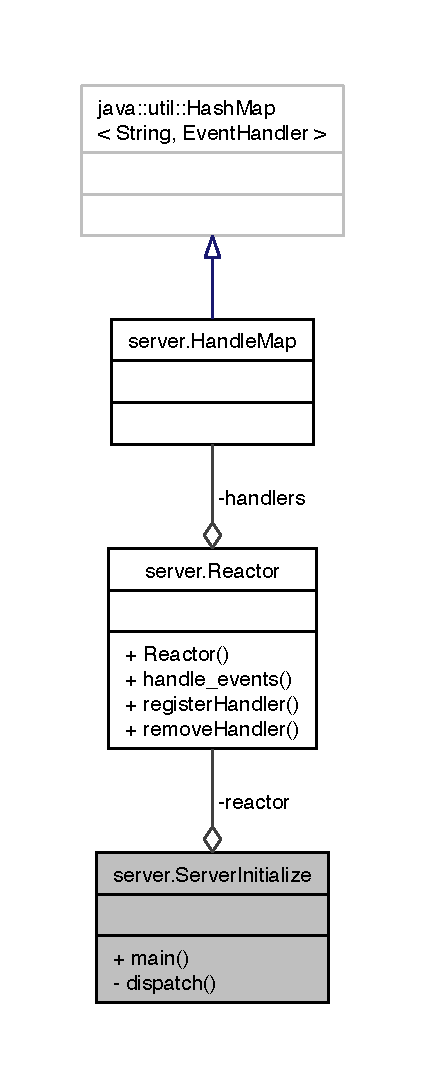
\includegraphics[width=204pt]{classserver_1_1_server_initialize__coll__graph}
\end{center}
\end{figure}
\subsection*{정적 Public 멤버 함수}
\begin{DoxyCompactItemize}
\item 
static void \hyperlink{classserver_1_1_server_initialize_ac00ce4d8c80d0da9e5c4011101f8ed28}{main} (String\mbox{[}$\,$\mbox{]} args)
\begin{DoxyCompactList}\small\item\em 메인 구문 \end{DoxyCompactList}\end{DoxyCompactItemize}
\subsection*{Private 멤버 함수}
\begin{DoxyCompactItemize}
\item 
void \hyperlink{classserver_1_1_server_initialize_aecdc0f2a4dbf79a19b710fda1fdcf554}{dispatch} ()
\begin{DoxyCompactList}\small\item\em Reactor를 실행한다. \end{DoxyCompactList}\end{DoxyCompactItemize}
\subsection*{Private 속성}
\begin{DoxyCompactItemize}
\item 
\hyperlink{classserver_1_1_reactor}{Reactor} \hyperlink{classserver_1_1_server_initialize_a16faf593fd3a106821a301c4d5089ee5}{reactor}
\end{DoxyCompactItemize}


\subsection{상세한 설명}
서버 초기화 클래스 

서버를 초기화하고 Reactor에 이벤트 핸들러를 등록한다. 

Server\-Initialize.\-java 파일의 12 번째 라인에서 정의되었습니다.



\subsection{멤버 함수 문서화}
\hypertarget{classserver_1_1_server_initialize_aecdc0f2a4dbf79a19b710fda1fdcf554}{\index{server\-::\-Server\-Initialize@{server\-::\-Server\-Initialize}!dispatch@{dispatch}}
\index{dispatch@{dispatch}!server::ServerInitialize@{server\-::\-Server\-Initialize}}
\subsubsection[{dispatch}]{\setlength{\rightskip}{0pt plus 5cm}void server.\-Server\-Initialize.\-dispatch (
\begin{DoxyParamCaption}
{}
\end{DoxyParamCaption}
)\hspace{0.3cm}{\ttfamily [private]}}}\label{classserver_1_1_server_initialize_aecdc0f2a4dbf79a19b710fda1fdcf554}


Reactor를 실행한다. 

Reactor를 초기화하고 이벤트 핸들러를 등록한다. Reactor에 이벤트 핸들링을 명령한다. \begin{DoxyReturn}{반환값}
Nothing 
\end{DoxyReturn}

\begin{DoxyExceptions}{예외}
{\em java.\-io.\-I\-O\-Exception} & 서버 소켓에서 I\-O 에러 발생 가능. \\
\hline
\end{DoxyExceptions}


Server\-Initialize.\-java 파일의 21 번째 라인에서 정의되었습니다.


\begin{DoxyCode}
21                             \{
22         \hyperlink{classserver_1_1_server_initialize_a16faf593fd3a106821a301c4d5089ee5}{reactor} = \textcolor{keyword}{new} Reactor();
23 
24         reactor.registerHandler(\textcolor{keyword}{new} SayHelloEventHandler());
25         reactor.registerHandler(\textcolor{keyword}{new} UpdateProfileEventHandler());
26 
27         \textcolor{keywordflow}{try} \{
28             reactor.handle\_events();
29         \} \textcolor{keywordflow}{catch} (IOException e) \{
30             e.printStackTrace();
31         \}
32     \}
\end{DoxyCode}
\hypertarget{classserver_1_1_server_initialize_ac00ce4d8c80d0da9e5c4011101f8ed28}{\index{server\-::\-Server\-Initialize@{server\-::\-Server\-Initialize}!main@{main}}
\index{main@{main}!server::ServerInitialize@{server\-::\-Server\-Initialize}}
\subsubsection[{main}]{\setlength{\rightskip}{0pt plus 5cm}static void server.\-Server\-Initialize.\-main (
\begin{DoxyParamCaption}
\item[{String\mbox{[}$\,$\mbox{]}}]{args}
\end{DoxyParamCaption}
)\hspace{0.3cm}{\ttfamily [static]}}}\label{classserver_1_1_server_initialize_ac00ce4d8c80d0da9e5c4011101f8ed28}


메인 구문 

Server를 초기화하고 Reactor에 전달한다. 
\begin{DoxyParams}{매개변수}
{\em args} & 기본 콘솔 변수 \\
\hline
\end{DoxyParams}
\begin{DoxyReturn}{반환값}
Nothing 
\end{DoxyReturn}


Server\-Initialize.\-java 파일의 40 번째 라인에서 정의되었습니다.


\begin{DoxyCode}
40                                            \{
41         ServerInitialize serverInitialize = \textcolor{keyword}{new} ServerInitialize();
42         serverInitialize.dispatch();
43     \}
\end{DoxyCode}


\subsection{멤버 데이타 문서화}
\hypertarget{classserver_1_1_server_initialize_a16faf593fd3a106821a301c4d5089ee5}{\index{server\-::\-Server\-Initialize@{server\-::\-Server\-Initialize}!reactor@{reactor}}
\index{reactor@{reactor}!server::ServerInitialize@{server\-::\-Server\-Initialize}}
\subsubsection[{reactor}]{\setlength{\rightskip}{0pt plus 5cm}{\bf Reactor} server.\-Server\-Initialize.\-reactor\hspace{0.3cm}{\ttfamily [private]}}}\label{classserver_1_1_server_initialize_a16faf593fd3a106821a301c4d5089ee5}


Server\-Initialize.\-java 파일의 13 번째 라인에서 정의되었습니다.



이 클래스에 대한 문서화 페이지는 다음의 파일로부터 생성되었습니다.\-:\begin{DoxyCompactItemize}
\item 
src/server/\hyperlink{_server_initialize_8java}{Server\-Initialize.\-java}\end{DoxyCompactItemize}

\chapter{파일 문서화}
\hypertarget{_main_8java}{\section{src/client/\-Main.java 파일 참조}
\label{_main_8java}\index{src/client/\-Main.\-java@{src/client/\-Main.\-java}}
}
\subsection*{클래스}
\begin{DoxyCompactItemize}
\item 
class \hyperlink{classclient_1_1_main}{client.\-Main}
\end{DoxyCompactItemize}
\subsection*{패키지}
\begin{DoxyCompactItemize}
\item 
package \hyperlink{namespaceclient}{client}
\end{DoxyCompactItemize}

\hypertarget{_demultiplexer_8java}{\section{src/server/\-Demultiplexer.java 파일 참조}
\label{_demultiplexer_8java}\index{src/server/\-Demultiplexer.\-java@{src/server/\-Demultiplexer.\-java}}
}
\subsection*{클래스}
\begin{DoxyCompactItemize}
\item 
class \hyperlink{classserver_1_1_demultiplexer}{server.\-Demultiplexer}
\begin{DoxyCompactList}\small\item\em 이벤트를 디코딩하여 적절한 핸들러에 전달한다. \end{DoxyCompactList}\end{DoxyCompactItemize}
\subsection*{패키지}
\begin{DoxyCompactItemize}
\item 
package \hyperlink{namespaceserver}{server}
\end{DoxyCompactItemize}

\hypertarget{_a_event_handler_8java}{\section{src/server/event\-\_\-handler/\-A\-Event\-Handler.java 파일 참조}
\label{_a_event_handler_8java}\index{src/server/event\-\_\-handler/\-A\-Event\-Handler.\-java@{src/server/event\-\_\-handler/\-A\-Event\-Handler.\-java}}
}
\subsection*{클래스}
\begin{DoxyCompactItemize}
\item 
class \hyperlink{classserver_1_1event__handler_1_1_a_event_handler}{server.\-event\-\_\-handler.\-A\-Event\-Handler}
\end{DoxyCompactItemize}
\subsection*{패키지}
\begin{DoxyCompactItemize}
\item 
package \hyperlink{namespaceserver_1_1event__handler}{server.\-event\-\_\-handler}
\end{DoxyCompactItemize}

\hypertarget{_b_event_handler_8java}{\section{src/server/event\-\_\-handler/\-B\-Event\-Handler.java 파일 참조}
\label{_b_event_handler_8java}\index{src/server/event\-\_\-handler/\-B\-Event\-Handler.\-java@{src/server/event\-\_\-handler/\-B\-Event\-Handler.\-java}}
}
\subsection*{클래스}
\begin{DoxyCompactItemize}
\item 
class \hyperlink{classserver_1_1event__handler_1_1_b_event_handler}{server.\-event\-\_\-handler.\-B\-Event\-Handler}
\end{DoxyCompactItemize}
\subsection*{패키지}
\begin{DoxyCompactItemize}
\item 
package \hyperlink{namespaceserver_1_1event__handler}{server.\-event\-\_\-handler}
\end{DoxyCompactItemize}

\hypertarget{_event_handler_8java}{\section{src/server/event\-\_\-handler/\-Event\-Handler.java 파일 참조}
\label{_event_handler_8java}\index{src/server/event\-\_\-handler/\-Event\-Handler.\-java@{src/server/event\-\_\-handler/\-Event\-Handler.\-java}}
}
\subsection*{클래스}
\begin{DoxyCompactItemize}
\item 
class \hyperlink{classserver_1_1event__handler_1_1_event_handler}{server.\-event\-\_\-handler.\-Event\-Handler}
\end{DoxyCompactItemize}
\subsection*{패키지}
\begin{DoxyCompactItemize}
\item 
package \hyperlink{namespaceserver_1_1event__handler}{server.\-event\-\_\-handler}
\end{DoxyCompactItemize}

\hypertarget{_handle_map_8java}{\section{src/server/\-Handle\-Map.java 파일 참조}
\label{_handle_map_8java}\index{src/server/\-Handle\-Map.\-java@{src/server/\-Handle\-Map.\-java}}
}
\subsection*{클래스}
\begin{DoxyCompactItemize}
\item 
class \hyperlink{classserver_1_1_handle_map}{server.\-Handle\-Map}
\begin{DoxyCompactList}\small\item\em 핸들과 이벤트 핸들러를 해쉬 형태로 저장하는 객체. \end{DoxyCompactList}\end{DoxyCompactItemize}
\subsection*{패키지}
\begin{DoxyCompactItemize}
\item 
package \hyperlink{namespaceserver}{server}
\end{DoxyCompactItemize}

\hypertarget{_reactor_8java}{\section{src/server/\-Reactor.java 파일 참조}
\label{_reactor_8java}\index{src/server/\-Reactor.\-java@{src/server/\-Reactor.\-java}}
}
\subsection*{클래스}
\begin{DoxyCompactItemize}
\item 
class \hyperlink{classserver_1_1_reactor}{server.\-Reactor}
\begin{DoxyCompactList}\small\item\em 이벤트 핸들러를 관리하는 객체. \end{DoxyCompactList}\end{DoxyCompactItemize}
\subsection*{패키지}
\begin{DoxyCompactItemize}
\item 
package \hyperlink{namespaceserver}{server}
\end{DoxyCompactItemize}

\hypertarget{_server_initialize_8java}{\section{src/server/\-Server\-Initialize.java 파일 참조}
\label{_server_initialize_8java}\index{src/server/\-Server\-Initialize.\-java@{src/server/\-Server\-Initialize.\-java}}
}
\subsection*{클래스}
\begin{DoxyCompactItemize}
\item 
class \hyperlink{classserver_1_1_server_initialize}{server.\-Server\-Initialize}
\end{DoxyCompactItemize}
\subsection*{패키지}
\begin{DoxyCompactItemize}
\item 
package \hyperlink{namespaceserver}{server}
\end{DoxyCompactItemize}

%--- End generated contents ---

% Index
\newpage
\phantomsection
\addcontentsline{toc}{chapter}{색인}
\printindex

\end{document}
